\chapter{Kwantummechanica voor chemici: modelsystemen}\label{ch:b3:quantum-model-systems}

Op een labtafel staan drie kolfjes, elk met een oplossing van een
cyaninekleurstof in ethanol: de eerste is magenta, de tweede blauw, de
derde diep groenblauw, met een absorptie in het verre rood. De drie
moleculen zijn op dezelfde manier gebouwd --- twee identieke
stikstofhoudende ringen, verbonden door een keten van koolstofatomen ---
en verschillen alleen in de lengte van die keten, telkens met twee
koolstofatomen. Hoe langer de keten, hoe verder de kleur naar het rood
verschuift. Een chemicus verklaarde de reeks in 1949 met een van de
eenvoudigste problemen van de kwantummechanica: een elektron dat vrij
kan bewegen langs een lijn van vaste lengte, een ``\omterm{def:b3:quantum-model-systems:box}{deeltje in een doos}''.
Dit hoofdstuk bouwt het gereedschap achter die verklaring op ---
\omterm{def:b3:quantum-model-systems:operator}{operatoren}, \omterm{def:b3:quantum-model-systems:operator}{eigenwaarden}, de \omterm{thm:b3:quantum-model-systems:schrodinger}{schrödingervergelijking} --- en lost de
modelsystemen op die de chemie elke dag gebruikt: de doos, de \omterm{def:b3:quantum-model-systems:oscillator}{harmonische
oscillator} van een trillende binding, de \omterm{def:b3:quantum-model-systems:rotor}{starre rotor} van een draaiend
molecuul, het waterstofatoom, en de barrière die een licht deeltje kan
passeren zonder de energie te hebben om erover te klimmen.

\begin{recall}
Het deel van jaar~1 liet zien dat de energie van een atoom gekwantiseerd
is (energieniveaus, grondtoestand en aangeslagen toestanden, de lijnen van
waterstof) en dat een foton de energie $E = h\nu = hc/\lambda$ draagt. Het
deel van jaar~2 beschreef een elektron met
een golffunctie $\psi$ waarvan het kwadraat een kansdichtheid is, splitste de
orbitalen van waterstof in een radiaal en een hoekafhankelijk deel en
telde hun knopen; de golffuncties van waterstof werden er als gegeven
aangenomen. Hier worden ze afgeleid, in paragraaf~5. Uit de natuurkunde:
de impuls $p = mv$ en de debroglie-golflengte
$\lambda = h/p$.
\end{recall}

\begin{omfigure}
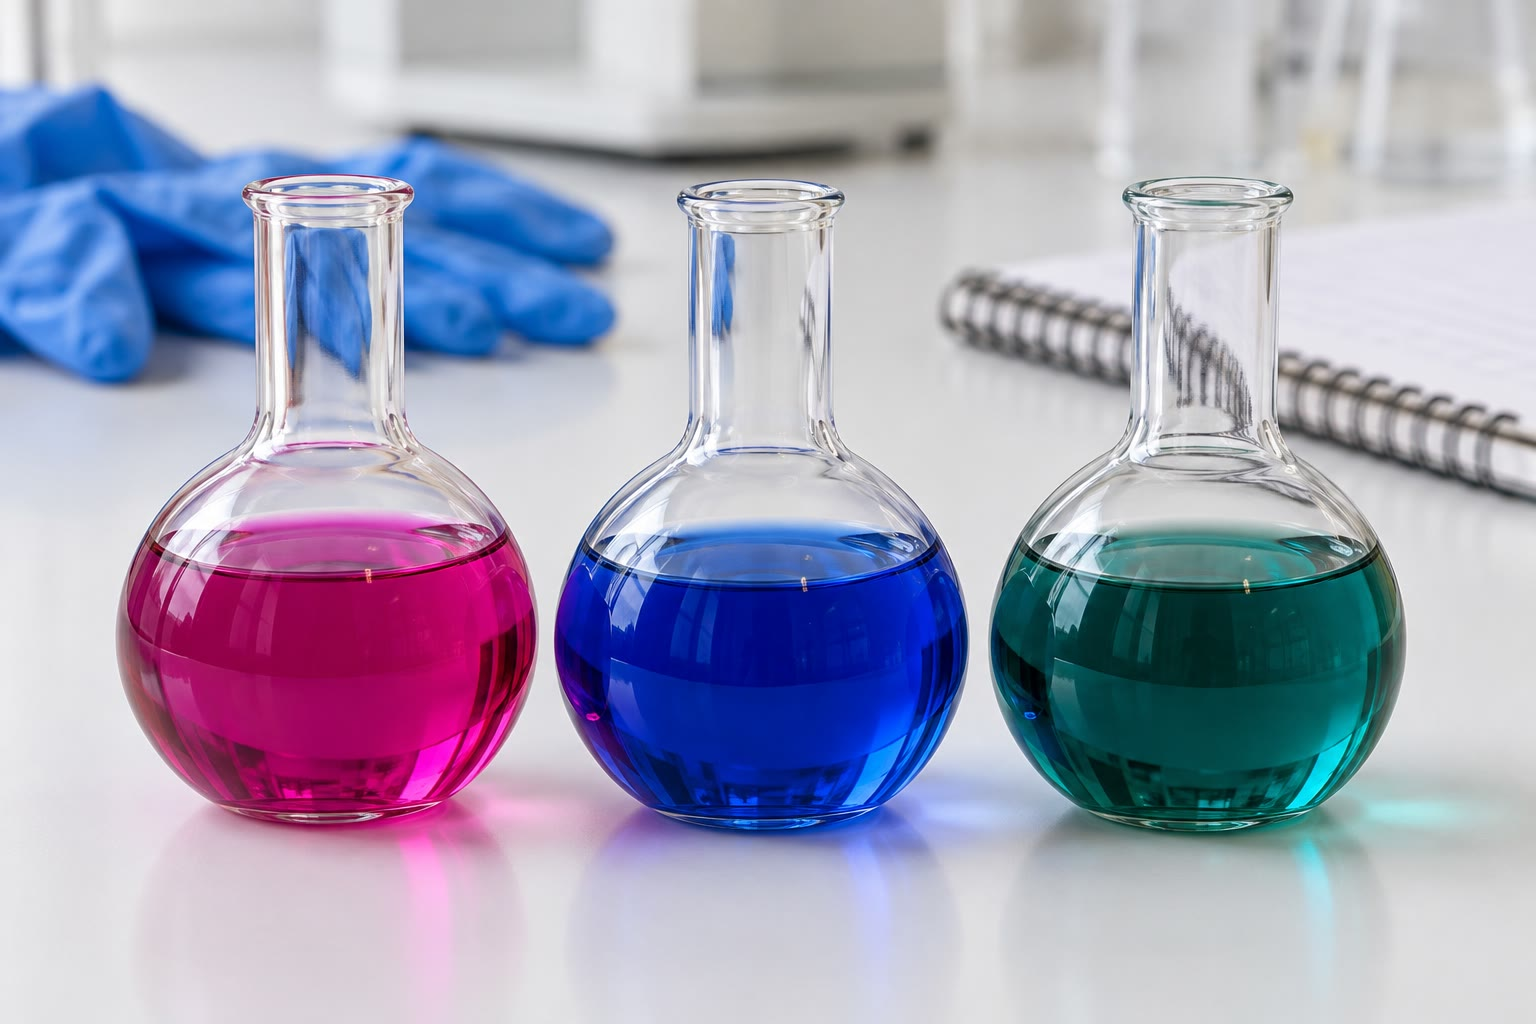
\includegraphics[width=0.62\linewidth]{images/book4/ai/b3-01-dyes.jpg}

{\small Oplossingen van drie cyaninekleurstoffen uit één familie. Elk
extra paar koolstofatomen in de keten verschuift de absorptie naar het
rood.}
\end{omfigure}

\section{Operatoren, eigenwaarden en de schrödingervergelijking}

De klassieke mechanica kent een deeltje op elk ogenblik een positie en een
impuls toe. De kwantummechanica kent het een toestand toe, de golffunctie
$\psi$, en vervangt elke meetbare grootheid door een bewerking op $\psi$.

\begin{definition}[Operator, eigenfunctie, eigenwaarde]\label{def:b3:quantum-model-systems:operator}
Een \emph{operator}\index{operator} $\hat A$ is een voorschrift dat een
functie omzet in een andere functie: $\hat A f = g$. Hij is lineair als $\hat A(\lambda f +
\mu g) = \lambda\hat Af + \mu\hat Ag$. Een functie $f$ die niet nul is en
waarvoor $\hat Af = a f$ voor een getal $a$, is een
\emph{eigenfunctie}\index{eigenfunctie} van $\hat A$, en $a$ is de
bijbehorende \emph{eigenwaarde}\index{eigenwaarde}.
\end{definition}

\begin{example}[Twee operatoren: positie en impuls]\label{ex:b3:quantum-model-systems:xp}
In één dimensie vermenigvuldigt de positieoperator met $x$, $\hat x f = xf$,
en differentieert de impulsoperator, $\hat p f = -\iu\hbar\,
\dd f/\dd x$, met $\hbar = h/2\pi$. De functie $\eu^{\iu kx}$ is een
\omterm{def:b3:quantum-model-systems:operator}{eigenfunctie} van $\hat p$ met \omterm{def:b3:quantum-model-systems:operator}{eigenwaarde} $\hbar k$: een golf met golflengte
$\lambda = 2\pi/k$ heeft impuls $h/\lambda$, de betrekking van De Broglie.
De functie $\sin kx$ is geen \omterm{def:b3:quantum-model-systems:operator}{eigenfunctie} van $\hat p$ (haar afgeleide is
een cosinus), maar wel van $\hat p^2 = -\hbar^2\,\dd^2/\dd x^2$, met
\omterm{def:b3:quantum-model-systems:operator}{eigenwaarde} $\hbar^2k^2$.
\end{example}

\begin{definition}[Hermitische operator, verwachtingswaarde]\label{def:b3:quantum-model-systems:hermitian}
Schrijf $\langle f|g\rangle = \int f^*g\,\dd\tau$ voor twee functies die op
de grenzen van het gebied nul worden. Een \omterm{def:b3:quantum-model-systems:operator}{operator} is
\emph{hermitisch}\index{hermitische operator}
als $\langle f|\hat Ag\rangle = \langle \hat Af|g\rangle$ voor alle zulke
$f$ en $g$. Voor een genormeerde toestand $\psi$ ($\langle\psi|\psi\rangle = 1$) is de
\emph{verwachtingswaarde}\index{verwachtingswaarde} van $\hat A$ gelijk aan
$\langle A\rangle = \langle\psi|\hat A\psi\rangle$: het gemiddelde van een
groot aantal metingen aan identiek geprepareerde systemen.
\end{definition}

De werkregels van de kwantumchemie --- haar postulaten --- passen nu in
één zin: elke meetbare grootheid wordt voorgesteld door een \omterm{def:b3:quantum-model-systems:hermitian}{hermitische
operator}; een meting levert een van zijn \omterm{def:b3:quantum-model-systems:operator}{eigenwaarden} op; en als
$\psi$ een \omterm{def:b3:quantum-model-systems:operator}{eigenfunctie} van $\hat A$ is, levert elke meting eraan dezelfde
waarde op, haar \omterm{def:b3:quantum-model-systems:operator}{eigenwaarde}.

\begin{theorem}[Hermitische operatoren]\label{thm:b3:quantum-model-systems:hermitian-real}
De \omterm{def:b3:quantum-model-systems:operator}{eigenwaarden} van een \omterm{def:b3:quantum-model-systems:hermitian}{hermitische operator} zijn reëel. Twee
\omterm{def:b3:quantum-model-systems:operator}{eigenfuncties} met verschillende \omterm{def:b3:quantum-model-systems:operator}{eigenwaarden} zijn orthogonaal:
$\langle f_1|f_2\rangle = 0$.
\end{theorem}

\begin{proof}
Stel $\hat Af = af$. Dan is $\langle f|\hat Af\rangle = a\langle f|f\rangle$ en
$\langle\hat Af|f\rangle = a^*\langle f|f\rangle$. De \omterm{def:b3:quantum-model-systems:operator}{operator} is \omterm{def:b3:quantum-model-systems:hermitian}{hermitisch},
dus beide zijn gelijk, en $\langle f|f\rangle > 0$: $a = a^*$. Stel nu $\hat Af_1
= a_1f_1$ en $\hat Af_2 = a_2f_2$ met $a_1 \ne a_2$, beide reëel. Dan is
$\langle f_1|\hat Af_2\rangle = a_2\langle f_1|f_2\rangle$ en $\langle\hat Af_1|
f_2\rangle = a_1\langle f_1|f_2\rangle$; hun gelijkheid geeft $(a_2 - a_1)
\langle f_1|f_2\rangle = 0$, dus $\langle f_1|f_2\rangle = 0$.
\end{proof}

Een meetwaarde is een reëel getal; daarom moeten waarneembare grootheden
\omterm{def:b3:quantum-model-systems:hermitian}{hermitisch} zijn. Orthogonaliteit maakt van de orbitalen van een atoom, of
de niveaus van een doos, een zuivere verzameling onafhankelijke
toestanden.

\begin{definition}[Commutator]\label{def:b3:quantum-model-systems:commutator}
De \emph{commutator}\index{commutator} van twee \omterm{def:b3:quantum-model-systems:operator}{operatoren} is $[\hat A,\hat B] =
\hat A\hat B - \hat B\hat A$. De \omterm{def:b3:quantum-model-systems:operator}{operatoren} commuteren als hun commutator
nul is.
\end{definition}

\begin{example}[De canonieke commutator]\label{ex:b3:quantum-model-systems:canonical}
Voor elke functie $f$ is $\hat x\hat pf = -\iu\hbar xf'$ en $\hat p\hat xf =
-\iu\hbar(f + xf')$. Het verschil is $[\hat x,\hat p]f = \iu\hbar f$, dus
$[\hat x,\hat p] = \iu\hbar$: positie en impuls commuteren niet. Deze ene
betrekking ligt ten grondslag aan het onzekerheidsprincipe en, verderop,
aan het volledige spectrum van de \omterm{def:b3:quantum-model-systems:oscillator}{harmonische oscillator}.
\end{example}

\begin{proposition}[Commuterende operatoren]\label{prop:b3:quantum-model-systems:commuting}
Als $\hat A$ en $\hat B$ commuteren en $f$ een \omterm{def:b3:quantum-model-systems:operator}{eigenfunctie} van $\hat A$ is
met een niet-ontaarde \omterm{def:b3:quantum-model-systems:operator}{eigenwaarde} $a$, dan is $f$ ook een \omterm{def:b3:quantum-model-systems:operator}{eigenfunctie} van
$\hat B$.
\end{proposition}

\begin{proof}
$\hat A(\hat Bf) = \hat B\hat Af = a(\hat Bf)$: de functie $\hat Bf$ is een
\omterm{def:b3:quantum-model-systems:operator}{eigenfunctie} van $\hat A$ met dezelfde \omterm{def:b3:quantum-model-systems:operator}{eigenwaarde} $a$, of nul. Omdat de
\omterm{def:b3:quantum-model-systems:operator}{eigenwaarde} niet ontaard is, is $\hat Bf$ een veelvoud van $f$, zeg $bf$.
\end{proof}

De \omterm{def:b3:quantum-model-systems:operator}{operator} van de energie is de \omterm{def:b3:quantum-model-systems:schrodinger}{hamiltonoperator}. Voor een deeltje met
massa $m$ in een potentiaal $V$ wordt de klassieke energie $p^2/2m + V$ een
\omterm{def:b3:quantum-model-systems:operator}{operator}.

\begin{definition}[Hamiltonoperator]\label{def:b3:quantum-model-systems:schrodinger}
De \emph{hamiltonoperator}\index{hamiltonoperator} van een deeltje met
massa $m$ dat beweegt in een potentiaal $V(\mathbf r)$ is
\[
\hat H = -\frac{\hbar^2}{2m}\nabla^2 + V(\mathbf r), \qquad \nabla^2 =
\frac{\partial^2}{\partial x^2} + \frac{\partial^2}{\partial y^2} +
\frac{\partial^2}{\partial z^2},
\]
en voor meerdere deeltjes de som van hun kinetische termen en van al hun
potentiële energieën.
\end{definition}

\begin{theorem}[De schrödingervergelijking]\label{thm:b3:quantum-model-systems:schrodinger}
De toestanden met een welbepaalde energie van een systeem --- zijn
stationaire toestanden --- zijn de \omterm{def:b3:quantum-model-systems:operator}{eigenfuncties} van zijn \omterm{def:b3:quantum-model-systems:schrodinger}{hamiltonoperator},
en zijn toegestane energieën zijn de \omterm{def:b3:quantum-model-systems:operator}{eigenwaarden}:
\[
\hat H\psi = E\psi,
\]
de tijdsonafhankelijke
\emph{schrödingervergelijking}\index{schrodingervergelijking@schrödingervergelijking}.
Een aanvaardbare $\psi$ is eenduidig, continu en kwadratisch integreerbaar
(ze kan genormeerd worden).
\end{theorem}
\begin{proof}[Status]
Dit is een postulaat, gerechtvaardigd door zijn gevolgen: de niveaus van
elk systeem dat hieronder wordt opgelost, stemmen overeen met de
spectroscopie. De tijdsafhankelijke vergelijking, waarvan dit het
stationaire geval is, hoort bij de natuurkunde.
\end{proof}

Het zijn de randvoorwaarden die kwantiseren: een differentiaalvergelijking
heeft oplossingen voor elke $E$, maar slechts een discrete verzameling
daarvan blijft eindig en continu. Chemie komt dan neer op een potentiaal
kiezen, oplossen en de \omterm{def:b3:quantum-model-systems:operator}{eigenwaarden} aflezen.

\begin{method}[Een eendimensionaal model oplossen]\label{met:b3:quantum-model-systems:one-dimensional}
\begin{enumerate}
  \item Schrijf de potentiaal $V(x)$ en de \omterm{def:b3:quantum-model-systems:schrodinger}{hamiltonoperator} op; verdeel de
        ruimte in gebieden waarin $V$ eenvoudig is.
  \item Los $-\frac{\hbar^2}{2m}\psi'' + V\psi = E\psi$ op in elk gebied: sinussen
        en cosinussen waar $E > V$, reële exponentiëlen waar $E < V$.
  \item Leg de voorwaarden op: $\psi = 0$ waar $V$ oneindig is; $\psi$
        en $\psi'$ continu bij een eindige sprong; $\psi \to 0$ op oneindig.
  \item Aan de voorwaarden is alleen voor bepaalde $E$ voldaan: dat zijn de
        niveaus.
  \item Normeer elke \omterm{def:b3:quantum-model-systems:operator}{eigenfunctie}; tel ter controle haar knopen (het
        $n$-de niveau van een eendimensionaal probleem heeft $n - 1$ knopen).
\end{enumerate}
\end{method}

\section{Het deeltje in een doos}

\begin{definition}[Deeltje in een doos, vrije-elektronenmodel]\label{def:b3:quantum-model-systems:box}
Een \emph{deeltje in een doos}\index{deeltje in een doos} beweegt vrij ($V = 0$)
tussen $x = 0$ en $x = L$ en kan niet ontsnappen ($V = \infty$ daarbuiten).
Het \emph{vrije-elektronenmodel}\index{vrije-elektronenmodel} van een
geconjugeerd molecuul behandelt zijn $\pi$-elektronen als onafhankelijke
deeltjes in een doos waarvan de lengte die van de geconjugeerde keten is.
\end{definition}

\begin{theorem}[Niveaus van de doos]\label{thm:b3:quantum-model-systems:box}
De niveaus en genormeerde \omterm{def:b3:quantum-model-systems:operator}{eigenfuncties} van een deeltje met massa $m$ in
een doos met lengte $L$ zijn
\[
E_n = \frac{n^2h^2}{8mL^2}, \qquad \psi_n(x) = \sqrt{\frac2L}\,\sin\frac{n\pi
x}{L}, \qquad n = 1, 2, 3, \dots
\]
\end{theorem}

\begin{proof}
Binnenin geldt $\psi'' = -k^2\psi$ met $k^2 = 2mE/\hbar^2$, dus $\psi = A\sin kx +
B\cos kx$. Buiten is $\psi = 0$ en continuïteit geeft $\psi(0) = 0$, dus $B =
0$, en $\psi(L) = 0$, dus $\sin kL = 0$ met $A \ne 0$: $kL = n\pi$, met $n$ een
positief geheel getal ($n = 0$ geeft $\psi = 0$; negatieve $n$ herhalen dezelfde
functies). Dan is $E = \hbar^2k^2/2m = n^2\pi^2\hbar^2/2mL^2 = n^2h^2/8mL^2$.
Ten slotte geeft $\int_0^L A^2\sin^2(n\pi x/L)\,\dd x = A^2L/2 = 1$ de waarde $A =
\sqrt{2/L}$.
\end{proof}

Drie kenmerken gelden voor elk gebonden systeem: de laagste energie is niet
nul (het deeltje is nooit in rust), de niveaus liggen verder uit elkaar
naarmate $n$ toeneemt, en ze komen dichter bij elkaar te liggen naarmate de
doos groter wordt ($E \propto 1/L^2$): een grote doos is bijna klassiek.

\begin{omfigure}
\begin{tikzpicture}
\begin{axis}[width=0.5\linewidth, height=6.4cm, xmin=-0.08, xmax=1.08,
  ymin=0, ymax=18.4, axis lines=left, xtick={0,1}, xticklabels={$0$,$L$},
  ytick={1,4,9,16}, yticklabels={$E_1$,$4E_1$,$9E_1$,$16E_1$},
  tick label style={font=\small}, xlabel={$x$}, title={\small $\psi_n$}]
\foreach \n in {1,4,9,16}{\addplot[gray!50, dashed, domain=0:1] {\n};}
\addplot[omDef, thick] table[x=x, y=p1] {figdata/out/bachelor-3-particle-in-box.dat};
\addplot[omDef, thick] table[x=x, y=p2] {figdata/out/bachelor-3-particle-in-box.dat};
\addplot[omDef, thick] table[x=x, y=p3] {figdata/out/bachelor-3-particle-in-box.dat};
\addplot[omDef, thick] table[x=x, y=p4] {figdata/out/bachelor-3-particle-in-box.dat};
\draw[very thick] (axis cs:0,0) -- (axis cs:0,18.4) (axis cs:1,0) -- (axis cs:1,18.4);
\end{axis}
\end{tikzpicture}\hspace{0.5em}%
\begin{tikzpicture}
\begin{axis}[width=0.5\linewidth, height=6.4cm, xmin=-0.08, xmax=1.08,
  ymin=0, ymax=18.4, axis lines=left, xtick={0,1}, xticklabels={$0$,$L$},
  ytick={1,4,9,16}, yticklabels={$n=1$,$n=2$,$n=3$,$n=4$},
  tick label style={font=\small}, xlabel={$x$}, title={\small $|\psi_n|^2$}]
\foreach \n in {1,4,9,16}{\addplot[gray!50, dashed, domain=0:1] {\n};}
\addplot[omThm, thick] table[x=x, y=d1] {figdata/out/bachelor-3-particle-in-box.dat};
\addplot[omThm, thick] table[x=x, y=d2] {figdata/out/bachelor-3-particle-in-box.dat};
\addplot[omThm, thick] table[x=x, y=d3] {figdata/out/bachelor-3-particle-in-box.dat};
\addplot[omThm, thick] table[x=x, y=d4] {figdata/out/bachelor-3-particle-in-box.dat};
\draw[very thick] (axis cs:0,0) -- (axis cs:0,18.4) (axis cs:1,0) -- (axis cs:1,18.4);
\end{axis}
\end{tikzpicture}

{\small De eerste vier niveaus van een \omterm{def:b3:quantum-model-systems:box}{deeltje in een doos}, elke functie
getekend op haar eigen niveau (gestippeld). Links: $\psi_n$, met $n - 1$
knopen binnen de doos. Rechts: de kansdichtheid $|\psi_n|^2$.}
\end{omfigure}

\begin{proposition}[De kubische doos]\label{prop:b3:quantum-model-systems:box-3d}
In een kubische doos met ribbe $L$ is $\psi = \psi_{n_x}(x)\psi_{n_y}(y)\psi_{n_z}(z)$ en
$E = (n_x^2 + n_y^2 + n_z^2)\,h^2/8mL^2$. Verschillende drietallen met dezelfde
som van kwadraten geven dezelfde energie.
\end{proposition}

\begin{proof}
Met $V = 0$ binnenin is $\hat H$ een som van drie eendimensionale
\omterm{def:b3:quantum-model-systems:operator}{operatoren}, één per coördinaat. Het product van drie eendimensionale
\omterm{def:b3:quantum-model-systems:operator}{eigenfuncties} is een \omterm{def:b3:quantum-model-systems:operator}{eigenfunctie} van de som, met als \omterm{def:b3:quantum-model-systems:operator}{eigenwaarde} de som
van de drie \omterm{def:b3:quantum-model-systems:operator}{eigenwaarden}; het wordt nul op elk zijvlak, zoals vereist.
\end{proof}

\begin{definition}[Ontaarde niveaus]\label{def:b3:quantum-model-systems:degenerate}
Lineair onafhankelijke \omterm{def:b3:quantum-model-systems:operator}{eigenfuncties} met dezelfde \omterm{def:b3:quantum-model-systems:operator}{eigenwaarde} zijn
\emph{ontaarde niveaus}\index{ontaarde niveaus}; hun aantal is de
\emph{ontaardingsgraad}\index{ontaardingsgraad} $g$ van die energie.
\end{definition}

\begin{example}[Ontaarding en symmetrie]\label{ex:b3:quantum-model-systems:cube}
Het niveau $n_x^2 + n_y^2 + n_z^2 = 6$ van de kubus komt van $(2,1,1)$,
$(1,2,1)$ en $(1,1,2)$: $g = 3$. Rek de doos een beetje uit langs $z$, en de
derde functie verwijdert zich van de andere twee: de ontaarding kwam voort
uit de symmetrie van de kubus. Hetzelfde verband tussen symmetrie en
ontaarding structureert \cref{ch:b3:point-groups,ch:b3:group-theory-applied}.
\end{example}

\subsection*{Geconjugeerde kleurstoffen}

In een symmetrische cyaninekleurstof verbindt een keten van $j$ atomen de
twee stikstofatomen
(\(j = 5\), 7, 9 voor de drie kleurstoffen uit de openingsscène), en de
$\pi$-elektronen zijn erover gedelokaliseerd. Een keten van $j$ atomen
draagt $N = j + 1$ $\pi$-elektronen: één per koolstofatoom, plus het vrije
elektronenpaar van één stikstofatoom, verdeeld over het hele kation.

\begin{proposition}[Absorptiegolflengte in het vrije-elektronenmodel]\label{prop:b3:quantum-model-systems:free-electron}
Als $N$ $\pi$-elektronen (een even aantal) de niveaus van een doos met
lengte $L$ vullen, twee per niveau, dan ligt de absorptie met de grootste
golflengte, van het hoogste bezette niveau $n = N/2$ naar het volgende, bij
\[
\lambda = \frac{8mcL^2}{h(N+1)}.
\]
\end{proposition}

\begin{proof}
$\Delta E = E_{N/2+1} - E_{N/2} = [(N/2+1)^2 - (N/2)^2]\,h^2/8mL^2 =
(N+1)\,h^2/8mL^2$, en $\lambda = hc/\Delta E$.
\end{proof}

\begin{example}[De kale doos faalt, een verlengde doos werkt]\label{ex:b3:quantum-model-systems:dyes}
% ledger: uvvis:cyanine, uvvis:carbocyanine, uvvis:dicarbocyanine, geo:C6H6.rCC
Neem elke binding van de keten gelijk aan de C--C-binding van benzeen,
$l = \qty{139.7}{pm}$, zodat de kale keten $(j - 1)l$ meet. Voor de
drie kleurstoffen ($N = 6$, 8, 10) geeft de formule 147, 257 en 374 nm, ver
onder de gemeten maxima van 524, 603 en 711 nm in ethanol. De elektronen
worden niet tegengehouden bij de stikstofatomen: ze lopen door in de
ringen. Verleng de doos aan elk uiteinde met een lengte $\delta$ en pas
$\delta$ aan op de middelste kleurstof:
$\delta = \qty{222}{pm}$, ongeveer anderhalve binding. Dezelfde $\delta$
voorspelt dan 474 en 732 nm voor de andere twee, binnen 10\,\% en 3\,\%. Eén
enkele aanpasbare lengte verklaart een hele familie van kleuren (figuur
hieronder; de getallen worden berekend in het script van de figuur).
\end{example}

\begin{omfigure}
\begin{tikzpicture}
\begin{axis}[width=0.5\linewidth, height=5.6cm, xmin=4, xmax=10,
  ymin=0, ymax=850, xtick={5,7,9}, axis lines=left,
  xlabel={atomen $j$ in de keten}, ylabel={$\lambda_{\max}$ / nm},
  legend cell align=left, legend style={font=\small, at={(1.03,0.5)}, anchor=west, draw=none},
  tick label style={font=\small}, label style={font=\small}]
\addplot[only marks, mark=*, omThm] table[x=j, y=measured] {figdata/out/bachelor-3-particle-in-box-dyes.dat};
\addlegendentry{gemeten (ethanol)}
\addplot[omDef, thick, mark=square*] table[x=j, y=fitted] {figdata/out/bachelor-3-particle-in-box-dyes.dat};
\addlegendentry{doos verlengd met $\delta = 222$ pm}
\addplot[gray, dashed, mark=triangle*] table[x=j, y=bare] {figdata/out/bachelor-3-particle-in-box-dyes.dat};
\addlegendentry{kale keten}
\end{axis}
\end{tikzpicture}

{\small Absorptiemaxima van de drie cyaninekleurstoffen tegenover het
\omterm{def:b3:quantum-model-systems:box}{vrije-elektronenmodel}: de kale keten, en de doos die aan elk uiteinde met
$\delta$ verlengd is, met $\delta$ aangepast op de middelste kleurstof.}
\end{omfigure}

\begin{inthelab}[Een reeks kleurstoffen meten]
De drie kleurstoffen worden afgewogen (enkele milligram), opgelost in
ethanol en verdund tot de absorbantie bij het maximum tussen 0.3 en 1
ligt. Van elke oplossing wordt het spectrum opgenomen tussen 400 en
800 nm in een cuvet van 1 cm, tegen een blanco van zuivere ethanol, en
$\lambda_{\max}$ wordt afgelezen aan de top van de hoofdband.
Cyaninekleurstoffen zijn sterk kleurende en irriterende vaste stoffen:
handschoenen dragen en afwegen in een zuurkast.
\end{inthelab}

\section{De harmonische oscillator}

Nabij de bodem van elke gladde potentiaalput geldt $V \approx \frac12 k(x - x_e)^2$:
kleine trillingen van een binding, van een atoom in een kristal of van een
molecuul in een kooi zijn alle bij benadering harmonisch.

\begin{definition}[Harmonische oscillator, krachtconstante, gereduceerde massa, nulpuntsenergie]\label{def:b3:quantum-model-systems:oscillator}
Een \emph{harmonische oscillator}\index{harmonische oscillator} is een
deeltje met massa $m$ in de potentiaal $V = \frac12 kx^2$; $k$ is de
\emph{krachtconstante}\index{krachtconstante}, en $\omega = \sqrt{k/m}$ de
klassieke hoekfrequentie. Een diatomisch molecuul met atoommassa's $m_1$, $m_2$
trilt als één deeltje met \emph{gereduceerde massa}\index{gereduceerde massa}
$\mu = m_1m_2/(m_1 + m_2)$ in de potentiaal van zijn binding. De energie van
het laagste niveau van een oscillator is zijn
\emph{nulpuntsenergie}\index{nulpuntsenergie}.
\end{definition}

\begin{definition}[Ladderoperatoren]\label{def:b3:quantum-model-systems:ladder}
Met $x_0 = \sqrt{\hbar/m\omega}$ zijn de
\emph{ladderoperatoren}\index{ladderoperatoren}
\[
\hat a = \frac{1}{\sqrt2}\Big(\frac{\hat x}{x_0} + \frac{\iu x_0\hat p}{\hbar}\Big),
\qquad \hat a^\dagger = \frac{1}{\sqrt2}\Big(\frac{\hat x}{x_0} -
\frac{\iu x_0\hat p}{\hbar}\Big).
\]
\end{definition}

\begin{theorem}[Niveaus van de harmonische oscillator]\label{thm:b3:quantum-model-systems:oscillator}
De niveaus van een \omterm{def:b3:quantum-model-systems:oscillator}{harmonische oscillator} zijn
\[
E_v = \big(v + \tfrac12\big)\hbar\omega = \big(v + \tfrac12\big)h\nu, \qquad v =
0, 1, 2, \dots,
\]
op gelijke afstanden $h\nu$ van elkaar, met de \omterm{def:b3:quantum-model-systems:oscillator}{nulpuntsenergie} $\frac12h\nu$.
\end{theorem}

\begin{proof}
Uit $[\hat x,\hat p] = \iu\hbar$ berekent men $[\hat a,\hat a^\dagger] = 1$ en
$\hat H = \hbar\omega(\hat a^\dagger\hat a + \frac12)$. Schrijf $\hat N =
\hat a^\dagger\hat a$. Dan is $[\hat N,\hat a] = -\hat a$ en $[\hat N,\hat
a^\dagger] = \hat a^\dagger$: als $\hat N\psi = \nu\psi$, dan is $\hat N(\hat
a\psi) = (\nu - 1)\hat a\psi$ en $\hat N(\hat a^\dagger\psi) = (\nu + 1)\hat
a^\dagger\psi$; $\hat a$ verlaagt de \omterm{def:b3:quantum-model-systems:operator}{eigenwaarde} met één, $\hat a^\dagger$
verhoogt ze. Maar $\nu = \langle\psi|\hat a^\dagger\hat a\psi\rangle/\langle\psi|\psi
\rangle = \|\hat a\psi\|^2/\|\psi\|^2 \ge 0$: de afdaling moet stoppen, en dat
gebeurt alleen bij een functie met $\hat a\psi_0 = 0$, met \omterm{def:b3:quantum-model-systems:operator}{eigenwaarde} $\nu = 0$.
De \omterm{def:b3:quantum-model-systems:operator}{eigenwaarden} van $\hat N$ zijn dus $v = 0, 1, 2, \dots$, en die van
$\hat H$ zijn $(v + \frac12)\hbar\omega$.
\end{proof}

\begin{proposition}[De eerste golffuncties]\label{prop:b3:quantum-model-systems:oscillator-functions}
In de gereduceerde coördinaat $y = x/x_0$ is
\[
\psi_0 \propto \eu^{-y^2/2}, \quad \psi_1 \propto 2y\,\eu^{-y^2/2}, \quad
\psi_2 \propto (4y^2 - 2)\eu^{-y^2/2}, \quad \psi_3 \propto (8y^3 -
12y)\eu^{-y^2/2},
\]
de hermitepolynomen maal een gaussfunctie. $\psi_v$ is even voor even $v$
en oneven voor oneven $v$.
\end{proposition}

\begin{proof}
$\hat a\psi_0 = 0$ luidt $y\psi_0 + \dd\psi_0/\dd y = 0$, met als oplossing de
gaussfunctie. Elke volgende functie is $\hat a^\dagger$ toegepast op de
vorige,
$\hat a^\dagger = \frac{1}{\sqrt2}(y - \dd/\dd y)$, wat het polynoom met $2y$
vermenigvuldigt en er zijn afgeleide van aftrekt: $1 \to 2y \to 4y^2 - 2 \to
8y^3 - 12y$ (op factoren na). De vervanging van $y$ door $-y$ verandert het
teken van $y$
en van $\dd/\dd y$, zodat $\hat a^\dagger$ bij elke stap de pariteit omkeert.
\end{proof}

\begin{omfigure}
\begin{tikzpicture}
\begin{axis}[width=0.66\linewidth, height=6.6cm, xmin=-4, xmax=4, ymin=0,
  ymax=4.6, axis lines=left, xlabel={$y = x/x_0$},
  ylabel={energie / $\hbar\omega$}, ytick={0.5,1.5,2.5,3.5},
  tick label style={font=\small}, label style={font=\small}]
\addplot[black, thick] table[x=y, y=V] {figdata/out/bachelor-3-harmonic-oscillator.dat};
\foreach \v in {0.5,1.5,2.5,3.5}{\addplot[gray!50, dashed, domain=-4:4] {\v};}
\addplot[omDef, thick] table[x=y, y=p0] {figdata/out/bachelor-3-harmonic-oscillator.dat};
\addplot[omDef, thick] table[x=y, y=p1] {figdata/out/bachelor-3-harmonic-oscillator.dat};
\addplot[omDef, thick] table[x=y, y=p2] {figdata/out/bachelor-3-harmonic-oscillator.dat};
\addplot[omDef, thick] table[x=y, y=p3] {figdata/out/bachelor-3-harmonic-oscillator.dat};
\addplot[only marks, mark=*, mark size=1.6pt, omThm] coordinates {(-1,0.5) (1,0.5)};
\node[omThm, font=\small, anchor=west] at (axis cs:2.0,0.2) {keerpunten};
\draw[omThm, ->, thin] (axis cs:2.0,0.2) -- (axis cs:1.08,0.47);
\end{axis}
\end{tikzpicture}

{\small De harmonische potentiaal, zijn eerste vier niveaus en
golffuncties, elk getekend op zijn niveau. De golffuncties reiken voorbij
de klassieke keerpunten ($y = \pm1$ voor $v = 0$, rode stippen), waar een
klassiek deeltje zou stilstaan.}
\end{omfigure}

\begin{example}[Nulpuntsenergieën van \ce{H2} en \ce{D2}]\label{ex:b3:quantum-model-systems:zpe}
% ledger: diat:H2.we, diat:D2.we
De harmonische golfgetallen zijn $\tilde\omega_e = \qty{4401.2}{cm^{-1}}$ voor
\ce{H2} en \qty{3115.5}{cm^{-1}} voor \ce{D2}, in de verhouding $1.413$, dicht bij
$\sqrt2$: dezelfde binding en \omterm{def:b3:quantum-model-systems:oscillator}{krachtconstante}, een verdubbelde \omterm{def:b3:quantum-model-systems:oscillator}{gereduceerde
massa}. De harmonische nulpuntsenergieën zijn de helft daarvan, 2200.6 en
\qty{1557.8}{cm^{-1}}, of
\qty{26.3}{kJ/mol} en \qty{18.6}{kJ/mol}. Een molecuul kan die energie
nooit kwijtraken; het verschil tussen isotopen is de bron van de
isotoopeffecten
van \cref{ch:b3:statistical-thermo-applied,ch:b3:rate-theories}.
\end{example}

\section{De starre rotor}

Een diatomisch molecuul draait ook om zijn massamiddelpunt. Opgevat als
twee massa's op een vaste afstand $r$ is het een \omterm{def:b3:quantum-model-systems:rotor}{starre rotor} met
traagheidsmoment
$I = \mu r^2$: de \omterm{def:b3:quantum-model-systems:oscillator}{gereduceerde massa} op afstand $r$ van de as.

\begin{definition}[Starre rotor, bolfuncties]\label{def:b3:quantum-model-systems:rotor}
Een \emph{starre rotor}\index{starre rotor} is een lichaam met een vaste
vorm dat vrij draait; voor een lineair molecuul is $\hat H = \hat L^2/2I$, waarbij $\hat L^2$ de
\omterm{def:b3:quantum-model-systems:operator}{operator} van het kwadraat van het impulsmoment is. Zijn \omterm{def:b3:quantum-model-systems:operator}{eigenfuncties}, die
alleen van de hoeken $\theta$ en $\phi$ afhangen, zijn de
\emph{bolfuncties}\index{bolfuncties} $Y_{l,m}(\theta,\phi)$, gelabeld met $l =
0, 1, 2, \dots$ en $m = -l, \dots, l$; voor een molecuul wordt $l$
geschreven als $J$.
\end{definition}

De rotor op een ring (rotatie in een vlak, om een vaste as) wordt eerst
opgelost; hij bevat de kern van de zaak.

\begin{theorem}[De ring]\label{thm:b3:quantum-model-systems:ring}
Een deeltje met traagheidsmoment $I$ dat in een vlak draait, heeft de
niveaus
$E_m = m^2\hbar^2/2I$ met $m = 0, \pm1, \pm2, \dots$; elk niveau behalve $m = 0$
is tweevoudig ontaard.
\end{theorem}

\begin{proof}
De enige coördinaat is de hoek $\phi$, en $\hat H = -(\hbar^2/2I)\,
\dd^2/\dd\phi^2$. De oplossingen van $\psi'' = -(2IE/\hbar^2)\psi$ zijn $\eu^{\iu
m\phi}$ met $m^2 = 2IE/\hbar^2$. Een eenduidige functie moet bij $\phi$ en
bij $\phi + 2\pi$ dezelfde waarde aannemen: $\eu^{2\pi\iu m} = 1$, dus $m$
is een geheel getal.
De functies met $m$ en $-m$ hebben dezelfde energie en zijn onafhankelijk.
\end{proof}

\begin{theorem}[Niveaus van de starre rotor]\label{thm:b3:quantum-model-systems:rotor}
$\hat L^2Y_{J,m} = J(J+1)\hbar^2\,Y_{J,m}$ en $\hat L_zY_{J,m} = m\hbar\,
Y_{J,m}$, zodat de niveaus van een lineaire \omterm{def:b3:quantum-model-systems:rotor}{starre rotor} gelijk zijn aan
\[
E_J = \frac{\hbar^2}{2I}\,J(J+1), \qquad J = 0, 1, 2, \dots,
\]
elk met \omterm{def:b3:quantum-model-systems:degenerate}{ontaardingsgraad} $g_J = 2J + 1$.
\end{theorem}
\admitted

Het algemene bewijs, met \omterm{def:b3:quantum-model-systems:ladder}{ladderoperatoren} voor het impulsmoment, hoort
thuis in meer gevorderde cursussen; hier volgt een controle. In
bolcoördinaten is
\[
\hat L^2 = -\hbar^2\Big[\frac{1}{\sin\theta}\frac{\partial}{\partial\theta}
\Big(\sin\theta\frac{\partial}{\partial\theta}\Big) +
\frac{1}{\sin^2\theta}\frac{\partial^2}{\partial\phi^2}\Big].
\]
Voor $Y_{1,0} \propto \cos\theta$ is de uitdrukking tussen haken $\frac{1}{\sin\theta}(-2\sin\theta
\cos\theta) = -2\cos\theta$, dus $\hat L^2Y_{1,0} = 2\hbar^2Y_{1,0} = 1(1+1)\hbar^2
Y_{1,0}$. Voor $Y_{1,\pm1} \propto \sin\theta\,\eu^{\pm\iu\phi}$ geeft
dezelfde berekening opnieuw $2\hbar^2$, en $\hat L_z = -\iu\hbar\,\partial/\partial
\phi$ geeft $\pm\hbar$.

\begin{proposition}[Reële bolfuncties]\label{prop:b3:quantum-model-systems:real-harmonics}
Voor $l = 1$ zijn de combinaties $Y_{1,0}$, $(Y_{1,-1} - Y_{1,1})/\sqrt2$ en
$\iu(Y_{1,-1} + Y_{1,1})/\sqrt2$ reëel en evenredig met $z/r$, $x/r$ en
$y/r$; voor $l = 2$ geeft dezelfde constructie functies die evenredig zijn
met $(3z^2 - r^2)$, $xz$, $yz$, $xy$ en $x^2 - y^2$, gedeeld door $r^2$.
\end{proposition}

\begin{proof}
$Y_{1,\pm1} \propto \mp\sin\theta\,\eu^{\pm\iu\phi}$ met de gebruikelijke
tekenconventie, zodat hun verschil gedeeld door $\sqrt2$ de vorm $\propto\sin\theta\cos\phi =
x/r$ heeft en de met $\iu$ gewogen som de vorm $\propto\sin\theta\sin\phi = y/r$;
$\cos\theta = z/r$. Elke combinatie van ontaarde \omterm{def:b3:quantum-model-systems:operator}{eigenfuncties} is nog
steeds een \omterm{def:b3:quantum-model-systems:operator}{eigenfunctie} van $\hat L^2$ (met dezelfde $l$), maar niet meer van $\hat
L_z$. Het geval $l = 2$ is dezelfde algebra met $\sin^2\theta\,\eu^{\pm2\iu\phi}$
en $\sin\theta\cos\theta\,\eu^{\pm\iu\phi}$.
\end{proof}

Dit zijn de hoekafhankelijke delen van de $p$- en $d$-orbitalen die in het
deel van jaar~2
getekend werden: hun namen $p_x$, $d_{xy}$, $d_{z^2}$ zijn de cartesische
vormen die we net vonden.

\begin{omfigure}
\begin{tikzpicture}[font=\small]
  \draw[->] (0,-0.2) -- (0,5.4) node[above] {$E/(\hbar^2/2I)$};
  \foreach \J/\E/\g in {0/0/1,1/2/3,2/6/5,3/12/7}{
    \pgfmathsetmacro{\y}{0.4*\E+0.1}
    \draw[omstate] (0.6,\y) -- (3.0,\y);
    \node[anchor=east] at (0.55,\y) {$\E$};
    \node[anchor=west] at (3.1,\y) {$J = \J$, \ $g = \g$};
  }
  \draw[<->, omThm] (2.4,0.9) -- (2.4,2.5) node[midway, left] {$4$};
  \draw[<->, omThm] (1.4,0.1) -- (1.4,0.9) node[midway, left] {$2$};
\end{tikzpicture}

{\small De eerste niveaus van een lineaire \omterm{def:b3:quantum-model-systems:rotor}{starre rotor}, $E_J = J(J+1)\,\hbar^2/2I$,
met hun ontaardingsgraden $2J + 1$. De tussenafstanden groeien als
$2(J+1)$: daarom liggen de lijnen van
\cref{ch:b3:rovibrational-spectroscopy} op gelijke afstanden.}
\end{omfigure}

\begin{example}[Rotatieniveaus van \ce{HCl}]\label{ex:b3:quantum-model-systems:hcl}
% ledger: diat:HCl.Be
Spectroscopisten schrijven $E_J = hcB\,J(J+1)$ met de rotatieconstante $B =
\hbar/(4\pi cI)$ in golfgetallen. Voor \ce{H^{35}Cl} is $B = \qty{10.593}{cm^{-1}}$:
de eerste niveaus liggen bij 0, 21.19, 63.56 en \qty{127.12}{cm^{-1}}, alle
ruim onder de thermische energie bij kamertemperatuur, $kT/hc = \qty{207}{cm^{-1}}$.
Veel rotatieniveaus zijn bezet; slechts één vibratieniveau is dat
($\tilde\omega_e = \qty{2991}{cm^{-1}}$).
\end{example}

\section{Het waterstofatoom en tunneling}

\subsection*{Het waterstofatoom, opgelost}

Een elektron met lading $-e$ rond een kern met lading $+e$ heeft $V = -e^2/
4\pi\varepsilon_0r$. Met de \omterm{def:b3:quantum-model-systems:oscillator}{gereduceerde massa} $\mu$ van elektron en proton is
\[
\hat H = -\frac{\hbar^2}{2\mu}\nabla^2 - \frac{e^2}{4\pi\varepsilon_0r},\qquad
\nabla^2 = \frac{1}{r^2}\frac{\partial}{\partial r}\Big(r^2\frac{\partial}{
\partial r}\Big) - \frac{\hat L^2}{\hbar^2r^2}.
\]
Het hoekafhankelijke deel van $\nabla^2$ is de rotoroperator: de
oplossingen
scheiden als $\psi = R(r)\,Y_{l,m}(\theta,\phi)$, en $R$ voldoet aan de
radiale vergelijking
\[
-\frac{\hbar^2}{2\mu}\frac{1}{r^2}\frac{\dd}{\dd r}\Big(r^2\frac{\dd R}{\dd r}
\Big) + \Big[\frac{l(l+1)\hbar^2}{2\mu r^2} - \frac{e^2}{4\pi\varepsilon_0r}
\Big]R = ER.
\]
De rotatie voegt een centrifugale term $l(l+1)\hbar^2/2\mu r^2$ toe die
elektronen met $l > 0$ weghoudt van de kern.

\begin{theorem}[Niveaus van het waterstofatoom]\label{thm:b3:quantum-model-systems:hydrogen}
De gebonden niveaus van een waterstofachtig atoom met kernlading $Ze$ zijn
\[
E_n = -\frac{\mu}{m_e}\,\frac{Z^2hcR_\infty}{n^2}, \qquad n = 1, 2, \dots,
\quad hcR_\infty = \frac{m_ee^4}{8\varepsilon_0^2h^2},
\]
met $l = 0, \dots, n - 1$; de radiale functies $1s$ en $2p$ zijn $R_{10}
\propto \eu^{-Zr/a}$ en $R_{21} \propto r\,\eu^{-Zr/2a}$, met $a =
(m_e/\mu)a_0$.
\end{theorem}

\begin{proof}[Gedeeltelijk bewijs]
Neem $Z = 1$ en probeer $R = \eu^{-r/a}$ met $l = 0$. Dan is $R' = -R/a$ en
$\frac{1}{r^2}(r^2R')' = R/a^2 - 2R/(ar)$. De radiale vergelijking wordt
$-\frac{\hbar^2}{2\mu}\big(\frac{1}{a^2} - \frac{2}{ar}\big) - \frac{e^2}{4\pi
\varepsilon_0r} = E$ voor alle $r$: de termen in $1/r$ vallen weg als $a =
4\pi\varepsilon_0\hbar^2/\mu e^2$, en dan is $E = -\hbar^2/2\mu a^2 = -\mu
e^4/8\varepsilon_0^2h^2$, het niveau $n = 1$. Met $R = r\eu^{-r/b}$ en $l = 1$
laat dezelfde substitutie termen in $1/r^2$ over (die wegvallen tegen de
centrifugale term), in $1/r$ (die wegvallen als $b = 2a$) en een constante, $E =
-\hbar^2/2\mu b^2$, een kwart van de vorige: het niveau $n = 2$. Het
algemene geval, een polynoom maal $\eu^{-r/na}$ waarvan de reeks moet
afbreken om normeerbaar te blijven, hoort thuis in meer gevorderde
cursussen.
\end{proof}

\begin{omfigure}
\begin{tikzpicture}
\begin{axis}[width=0.66\linewidth, height=5.4cm, xmin=0, xmax=12,
  ymin=-0.15, ymax=1.05, axis lines=left, samples=160, domain=0:12,
  xlabel={$r/a$}, ylabel={$R(r)$, geschaald},
  legend cell align=left, legend style={font=\small, draw=none}, tick label style={font=\small},
  label style={font=\small}]
\addplot[omDef, thick] {exp(-x)}; \addlegendentry{$R_{10} \propto \eu^{-r/a}$}
\addplot[omThm, thick] {(1-x/2)*exp(-x/2)}; \addlegendentry{$R_{20} \propto (1 - r/2a)\eu^{-r/2a}$}
\addplot[omProp, thick] {0.5*x*exp(-x/2)/exp(-1)}; \addlegendentry{$R_{21} \propto r\,\eu^{-r/2a}$}
\addplot[gray, dashed] {0};
\end{axis}
\end{tikzpicture}

{\small Radiale functies van het waterstofatoom, uit de oplossingen
hierboven (elk geschaald tot een maximum van ongeveer 1). $R_{20}$ heeft
één radiale knoop bij $r = 2a$; $R_{21}$ is nul in de kern, naar buiten
gedreven door de centrifugale term.}
\end{omfigure}

\begin{example}[De ionisatie-energie van waterstof]\label{ex:b3:quantum-model-systems:ie}
% ledger: const:RyhcEV, const:me, const:mp
$hcR_\infty = \qty{13.6057}{eV}$ en $\mu/m_e = 1/(1 + m_e/m_p) = 0.999456$, dus
$-E_1 = \qty{13.598}{eV}$: de gemeten ionisatie-energie van waterstof, tot
op het laatste cijfer dat het deel van jaar~1 gaf. De \omterm{def:b3:quantum-model-systems:oscillator}{gereduceerde massa}
verandert het vierde significante cijfer.
\end{example}

\subsection*{Tunneling}

\begin{definition}[Tunneling, transmissiekans]\label{def:b3:quantum-model-systems:tunnelling}
Men spreekt van \emph{tunneling}\index{tunneling} wanneer een deeltje een
gebied doorkruist waar zijn energie lager is dan de potentiële energie,
wat in de klassieke mechanica verboden is. De
\emph{transmissiekans}\index{transmissiekans}
$T$ van een barrière is de fractie van de invallende deeltjes die erachter
wordt aangetroffen.
\end{definition}

\begin{proposition}[Dunne en dikke barrières]\label{prop:b3:quantum-model-systems:barrier}
Binnen een barrière met hoogte $V_0 > E$ is $\psi$ een combinatie van
$\eu^{\pm\kappa x}$ met $\kappa = \sqrt{2m(V_0 - E)}/\hbar$. Voor een
rechthoekige barrière met breedte $a$ is
\[
T = \Big[1 + \frac{\sinh^2(\kappa a)}{4\varepsilon(1-\varepsilon)}\Big]^{-1},
\qquad \varepsilon = \frac{E}{V_0},
\]
en voor een dikke barrière ($\kappa a \gg 1$) is $T \approx 16\varepsilon(1-\varepsilon)
\,\eu^{-2\kappa a}$.
\end{proposition}

\begin{proof}[Gedeeltelijk bewijs]
In de barrière luidt de \omterm{thm:b3:quantum-model-systems:schrodinger}{schrödingervergelijking} $\psi'' = \kappa^2\psi$, met
als oplossingen de twee exponentiëlen. Het aansluiten van $\psi$ en
$\psi'$ op de twee wanden met de golven $\eu^{\pm\iu kx}$ buiten de
barrière geeft vier lineaire vergelijkingen; hun
oplossing, een bladzijde algebra, is de formule voor $T$, die hier wordt
aangenomen. Voor grote $\kappa a$ domineert $\sinh\kappa a \approx \frac12\eu^{\kappa a}$, wat
de vorm voor een dikke barrière geeft.
\end{proof}

De doorslaggevende factor is $\eu^{-2\kappa a}$, en $\kappa \propto \sqrt m$:
\omterm{def:b3:quantum-model-systems:tunnelling}{tunneling} is een zaak van de lichtste deeltjes, eerst elektronen, dan
protonen, en veel minder deuteronen.

\begin{omfigure}
\begin{tikzpicture}
\begin{axis}[width=0.66\linewidth, height=5.6cm, xmin=0, xmax=1, ymode=log,
  ymin=1e-10, ymax=1e-1, axis lines=left, xlabel={$E/V_0$},
  ylabel={transmissiekans $T$},
  legend cell align=left, legend style={font=\small, at={(0.03,0.97)}, anchor=north west, draw=none},
  tick label style={font=\small}, label style={font=\small}]
\addplot[omDef, thick] table[x=eps, y=TH] {figdata/out/bachelor-3-tunnelling.dat};
\addlegendentry{proton}
\addplot[omThm, thick, dashed] table[x=eps, y=TD] {figdata/out/bachelor-3-tunnelling.dat};
\addlegendentry{deuteron}
\end{axis}
\end{tikzpicture}

{\small \omterm{def:b3:quantum-model-systems:tunnelling}{Transmissiekans} door een modelbarrière van 0.40 eV hoog en
50 pm breed. Bij de halve barrièrehoogte gaat het proton ongeveer 58 keer
vaker door dan het deuteron (logaritmische schaal).}
\end{omfigure}

\begin{remark}[Waar tunneling zichtbaar wordt]\label{rem:b3:quantum-model-systems:where}
Het ammoniakmolecuul klapt binnenstebuiten, waarbij het stikstofatoom door
het vlak van de drie waterstofatomen gaat, door te tunnelen door een lage
barrière; overdrachten van protonen en waterstofatomen in enzymen vertonen
kinetische isotoopeffecten die veel groter zijn dan
\cref{ch:b3:rate-theories} zonder \omterm{def:b3:quantum-model-systems:tunnelling}{tunneling} voorspelt; en de
rastertunnelmicroscoop beeldt afzonderlijke atomen op een oppervlak af met
de stroom van elektronen die door een vacuümspleet van enkele tienden van
een nanometer tunnelen, een stroom die tien keer kleiner wordt bij elke
extra 0.1 nm.
\end{remark}

\begin{history}[Schrödinger, 1926]
\begin{minipage}[t]{0.72\linewidth}
In vier artikelen uit de eerste helft van 1926 verving Erwin Schrödinger
de kwantumregels van het atoom van Bohr door een golfvergelijking, loste
hij die op voor het waterstofatoom, de oscillator en de rotor, en vond hij
de niveaus terug die de spectroscopie had gemeten. De gehele getallen die
Bohr met de hand had opgelegd, verschenen nu vanzelf, even natuurlijk als
het aantal knopen van een trillende snaar.
Hij deelde de Nobelprijs voor de Natuurkunde van 1933 met Paul Dirac.
\end{minipage}\hfill
\begin{minipage}[t]{0.22\linewidth}\vspace{0pt}
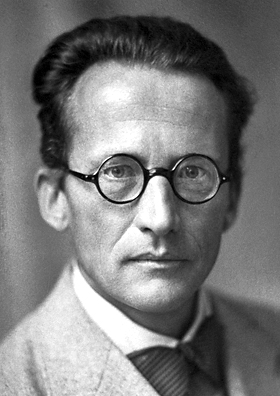
\includegraphics[width=\linewidth]{images/book4/schrodinger-1933.jpg}\par
{\footnotesize Schrödinger in 1933.}
\end{minipage}
\end{history}

\section{Oefeningen}

\begin{exercise}[$\star$]\label{exo:b3:quantum-model-systems:1}
Een elektron is opgesloten in een doos met lengte (a) \qty{1.00}{nm}, (b)
\qty{0.50}{nm}. Bereken $E_1$ in joule en in elektronvolt, en de golflengte
van de overgang $n = 1 \to 2$.
\end{exercise}

\begin{exercise}[$\star$]\label{exo:b3:quantum-model-systems:2}
Geef de vijf laagste niveaus van een deeltje in een kubische doos, in
eenheden van
$h^2/8mL^2$, met hun ontaardingsgraden.
\end{exercise}

\begin{exercise}[$\star$]\label{exo:b3:quantum-model-systems:3}
Bereken de \omterm{def:b3:quantum-model-systems:commutator}{commutatoren} $[\hat x^2,\hat p]$ en $[\hat p^2,\hat x]$ door ze
te laten inwerken op een functie $f(x)$.
\end{exercise}

\begin{exercise}[$\star$]\label{exo:b3:quantum-model-systems:4}
% ledger: diat:HCl.Be
Geef met $B = \qty{10.593}{cm^{-1}}$ voor \ce{H^{35}Cl} de energieën (in
\unit{cm^{-1}}) en ontaardingsgraden van de niveaus $J = 0$ tot 3, en het
traagheidsmoment van het molecuul.
\end{exercise}

\begin{exercise}[$\star\star$]\label{exo:b3:quantum-model-systems:5}
Bereken voor de toestand $\psi_n$ van een \omterm{def:b3:quantum-model-systems:box}{deeltje in een doos} $\langle x\rangle$ en
$\langle x^2\rangle$. Bereken $\langle x^2\rangle$ voor $n = 1$ en vergelijk met
de klassieke waarde $L^2/3$ voor een deeltje dat zich met gelijke kans
overal kan bevinden.
\end{exercise}

\begin{exercise}[$\star\star$]\label{exo:b3:quantum-model-systems:6}
% ledger: diat:H2.we, diat:D2.we
Bereken de harmonische nulpuntsenergieën van \ce{H2} en \ce{D2} in
\unit{kJ/mol} uit $\tilde\omega_e = \qty{4401.2}{cm^{-1}}$ en
\qty{3115.5}{cm^{-1}}, en hun verschil. Welke verhouding van golfgetallen
verwacht je op grond van de \omterm{def:b3:quantum-model-systems:oscillator}{gereduceerde massa}'s, en hoe dicht ligt de
gemeten verhouding daarbij?
\end{exercise}

\begin{exercise}[$\star\star$]\label{exo:b3:quantum-model-systems:7}
De functie $\phi = Nx(L - x)$ is een ruwe gok voor de grondtoestand van de
doos. Normeer haar en bereken daarna haar overlap $\langle\psi_1|\phi\rangle$ met
de echte grondtoestand.
\end{exercise}

\begin{exercise}[$\star\star$]\label{exo:b3:quantum-model-systems:8}
Toon aan dat $\hat p = -\iu\hbar\,\dd/\dd x$ \omterm{def:b3:quantum-model-systems:hermitian}{hermitisch} is voor functies die
nul worden aan de uiteinden van een interval, en dat $\hat x\hat p$ dat niet is.
\end{exercise}

\begin{exercise}[$\star\star$]\label{exo:b3:quantum-model-systems:9}
Modelleer hexa-1,3,5-trieen als zes $\pi$-elektronen in een doos met
lengte $6l$, $l =
\qty{139.7}{pm}$ (vijf bindingen en een halve binding aan elk uiteinde).
Voorspel de golflengte van zijn eerste absorptie. Is het molecuul gekleurd?
\end{exercise}

\begin{exercise}[$\star\star\star$]\label{exo:b3:quantum-model-systems:10}
Bereken voor de modelbarrière van de figuur ($V_0 = \qty{0.40}{eV}$, $a = \qty{50}{pm}$)
bij $E = V_0/2$ de grootheid $\kappa$ voor een proton en een deuteron en,
met de formule voor een dikke barrière, de verhouding $T_H/T_D$. Vergelijk
met de exacte verhouding, 58.
\end{exercise}

\begin{exercise}[$\star\star\star$]\label{exo:b3:quantum-model-systems:11}
Behandel de zes $\pi$-elektronen van benzeen als deeltjes op een ring met
straal
\qty{139.7}{pm} (de C--C-afstand is gelijk aan de straal van een regelmatige
zeshoek). Vul de niveaus en bereken daarna de golflengte van de overgang
van het hoogste bezette naar het laagste lege niveau.
\end{exercise}

\begin{exercise}[$\star\star\star$]\label{exo:b3:quantum-model-systems:12}
Voor de $1s$-toestand van waterstof is $\psi = (\pi a^3)^{-1/2}\eu^{-r/a}$.
Bereken de \omterm{def:b3:quantum-model-systems:hermitian}{verwachtingswaarden} $\langle r\rangle$ en $\langle V\rangle$, en
controleer dat
$\langle V\rangle = 2E_1$. (Gebruik $\int_0^\infty r^n\eu^{-\beta r}\dd r =
n!/\beta^{n+1}$.)
\end{exercise}

\section{Probleem: hoe lang is een kleurstof?}

\begin{problem}[{Weekendprobleem --- het vrije-elektronenmodel van drie
cyaninekleurstoffen: waarom een kale keten faalt, welke overgangen
toegestaan zijn, de energieschalen van een molecuul, en de doos die past}]
\label{pb:b3:quantum-model-systems:1}
% ledger: uvvis:cyanine, uvvis:carbocyanine, uvvis:dicarbocyanine, geo:C6H6.rCC, diat:HCl.we, diat:HCl.Be
Drie symmetrische cyaninekleurstoffen absorberen bij 524, 603 en 711 nm in
ethanol; hun geconjugeerde ketens, tussen en met inbegrip van de twee
stikstofatomen, tellen $j = 5$, 7
en 9 atomen. Neem elke binding gelijk aan $l = \qty{139.7}{pm}$, $m_e =
\qty{9.109e-31}{kg}$, $h = \qty{6.626e-34}{J.s}$, $c = \qty{2.998e8}{m/s}$,
$k = \qty{1.381e-23}{J/K}$, $\qty{1}{eV} = \qty{1.602e-19}{J}$.

\medskip\noindent\textbf{Deel I --- Een kale keten.}
\begin{enumerate}
  \item Leg uit waarom een keten van $j$ atomen $N = j + 1$ $\pi$-elektronen
        draagt, en geef $N$ voor elke kleurstof.
  \item Welke niveaus van de doos zijn voor de eerste kleurstof het hoogste
        bezette en het laagste lege?
  \item Toon aan dat de eerste absorptie ligt bij $\lambda = 8mcL^2/h(N+1)$.
  \item Geef de kale lengte $L_0 = (j - 1)l$ van elke keten.
  \item Bereken $\lambda$ voor elke kleurstof met $L = L_0$.
  \item Vergelijk met de gemeten waarden. In welke richting zit het model
        ernaast, en wat zegt dat over $L$?
\end{enumerate}

\medskip\noindent\textbf{Deel II --- Welke overgangen toegestaan zijn.}
De intensiteit van een overgang $n \to n'$ is evenredig met $|\langle
\psi_n|x - L/2|\psi_{n'}\rangle|^2$.
\begin{enumerate}[resume]
  \item Toon aan dat $\psi_n$ symmetrisch is ten opzichte van het midden van
        de doos voor oneven $n$ en antisymmetrisch voor even $n$.
  \item Leid af dat de integraal nul is wanneer $n + n'$ even is.
  \item Is de overgang HOMO $\to$ LUMO van elke kleurstof toegestaan?
  \item Is voor de tweede kleurstof de overgang van de HOMO naar het niveau
        boven de LUMO toegestaan? En die van het niveau onder de HOMO naar de LUMO?
  \item Bij welke golflengte (als fractie van de eerste) zou in het model
        de volgende toegestane overgang vanuit de HOMO liggen?
  \item Waarom overleeft zo'n regel, die alleen uit de symmetrie volgt, de
        grofheid van het model?
\end{enumerate}

\medskip\noindent\textbf{Deel III --- De energieschalen van een molecuul.}
\begin{enumerate}[resume]
  \item Zet de absorptie van de tweede kleurstof om in een energie in eV.
  \item De vibratie van \ce{HCl} heeft $\tilde\omega_e = \qty{2991}{cm^{-1}}$:
        zet haar kwantum om in eV.
  \item De rotatie van \ce{HCl} heeft $B = \qty{10.59}{cm^{-1}}$: zet de
        afstand tussen $J = 0$ en $J = 1$ om in meV.
  \item Bereken $kT$ in meV bij \qty{298}{K}.
  \item Welke soorten excitatie zijn bij kamertemperatuur bezet?
  \item In welke gebieden van het spectrum worden elektronische, vibratie-
        en rotatieovergangen waargenomen?
\end{enumerate}

\medskip\noindent\textbf{Deel IV --- De doos die past.}
\begin{enumerate}[resume]
  \item Bereken uit de gemeten 603 nm de lengte $L$ die de doos van de
        tweede kleurstof moet hebben.
  \item Schrijf $L = L_0 + 2\delta$ en leid $\delta$ af.
  \item Voorspel met deze $\delta$ de waarde van $\lambda$ voor de eerste
        kleurstof; geef de relatieve fout.
  \item Dezelfde vraag voor de derde kleurstof.
  \item Interpreteer $\delta$: waar gaan de $\pi$-elektronen voorbij de
        stikstofatomen naartoe?
  \item Druk $\delta$ uit in bindingslengtes en formuleer het resultaat van
        het probleem: de effectieve verlenging van de doos aan elk uiteinde.
\end{enumerate}
\end{problem}
